\documentclass[a4paper,11pt]{article}

%!TEX root = HDR.tex

%%%%%%%%%%%%%%%% FONTS %%%%%%%%%%%%%%%%
\usepackage{amsmath} % required by mathspec
\usepackage{mathspec} % includes fontspec

	% undo wrong change made by mathspec (cf link below)
	\makeatletter
	\let\RequirePackage\original@RequirePackage
	\let\usepackage\RequirePackage
	\makeatother
	% https://tex.stackexchange.com/questions/85696/what-causes-this-strange-interaction-between-glossaries-and-amsmath

\setmainfont[%
	WordSpace=1.25,
	]{STIX Two Text}[]

%\setsansfont[%
%	WordSpace=1.5,
%	Scale=MatchLowercase,%
%	UprightFont = FiraGO Regular,%
%	BoldFont = FiraGO Medium,%
%	ItalicFont = FiraGO Italic,%
%	BoldItalicFont = FiraGO Medium Italic%
%	]{FiraGO}

\setsansfont[%
	WordSpace=1.25,
	Scale=MatchLowercase,%
	]{Source Sans 3}

\setmonofont[%
	WordSpace=1.25,
	Scale=MatchLowercase,%
	UprightFont = JetBrains Mono Regular,%
	BoldFont = JetBrains Mono Bold,%
	ItalicFont = JetBrains Mono Italic,%
	BoldItalicFont = JetBrains Mono Bold Italic,%
%	Color = 008800,%
	]{JetBrains Mono}

%%%%%%%%%%%%%%%% MATHS %%%%%%%%%%%%%%%%
\usepackage{mathtools}
\usepackage{amssymb}
\usepackage{nicefrac}
\setmathfont(Digits,Latin,Greek)[
	UprightFont    = STIX Two Text,
	BoldFont       = STIX Two Text Bold,
	ItalicFont     = STIX Two Text Italic,
	BoldItalicFont = STIX Two Text Bold Italic,
	Numbers        = Lining
	]{STIX Two Text}
	
\setmathrm[
	Scale=MatchLowercase,%
	UprightFont    = STIX Two Text,
	BoldFont       = STIX Two Text Bold,
	ItalicFont     = STIX Two Text Italic,
	BoldItalicFont = STIX Two Text Bold Italic,
	Numbers        = Lining
	]{STIX Two Text}
%\setmathsf[
%	Scale=MatchLowercase,%
%	]{Fira Math}

	% additional mathspec corrections (cf link below)
	\makeatletter
	\ernewcommand\eu@MathPunctuation@symfont{Latin:m:n}
	\DeclareMathSymbol{,}{\mathpunct}{\eu@MathPunctuation@symfont}{`,}
	\DeclareMathSymbol{.}{\mathord}{\eu@MathPunctuation@symfont}{`.}
	\DeclareMathSymbol{<}{\mathrel}{\eu@MathPunctuation@symfont}{`<}
	\DeclareMathSymbol{>}{\mathrel}{\eu@MathPunctuation@symfont}{`>}
	\DeclareMathSymbol{/}{\mathord}{\eu@MathPunctuation@symfont}{`/}
	\DeclareMathSymbol{;}{\mathpunct}{\eu@MathPunctuation@symfont}{`;}
	\XeTeXDeclareMathSymbol{^^^^2026}{\mathinner}{\eu@MathPunctuation@symfont}{"2026}[\mathellipsis]
	\makeatother
	% https://tex.stackexchange.com/questions/74140/xetex-mathspec-punctuation-issue

%%%%%%%%%%%%%%%% TYPOGRAPHY %%%%%%%%%%%%%%%%
\usepackage[stretch=10]{microtype}
\usepackage[defaultlines=2,all]{nowidow}

\usepackage{etoolbox}
\makeatletter
\preto{\@verbatim}{\topsep=1ex \partopsep=1ex \color[rgb]{.3,.3,.3}}
\makeatother
\usepackage{booktabs}
\usepackage{fontawesome5}
\usepackage[text={160mm,250mm},centering,top=20mm,footskip=15mm]{geometry}


\usepackage{titlesec}

\titleformat%
{\section}% command
[block]% shape
{\sffamily\bfseries\Large}% format
{\thesection}% label
{1em}% separation
{}% before-code
[]% after-code

\titleformat%
{\subsection}% command
[block]% shape
{\sffamily\bfseries\large}% format
{\thesection}% label
{1em}% separation
{}% before-code
[]% after-code

\titleformat%
{\subsubsection}% command
[block]% shape
{\sffamily\bfseries\normalsize}% format
{\thesection}% label
{1em}% separation
{}% before-code
[]% after-code

\usepackage[font=footnotesize, labelfont=bf, labelsep=endash]{caption}
\usepackage[skip,indent]{parskip}

\usepackage[backend=biber,
%            dashed=true,
            maxcitenames=2,
            sorting=none,
            uniquelist=false,
            maxbibnames=99,
            firstinits=false,
            isbn=false,
            doi=true,
            url=true,
            sortcites=true,
            defernumbers=true,
            abbreviate=false,
			autocite=footnote,
            style=ext-numeric-comp]{biblatex} 

%%-- formatting hell for biblatex

%-- citations with square brackets
\DeclareOuterCiteDelims{parencite}{\bibopenbracket}{\bibclosebracket}
\DeclareInnerCiteDelims{textcite}{\bibopenbracket}{\bibclosebracket}

%%-- remove "In:"
\renewbibmacro{in:}{}

%%-- no "quotes" around titles of chapters/article titles
\DeclareFieldFormat[article, inbook, incollection, inproceedings, misc, thesis, unpublished]
{title}{#1}

%%-- no punctuation after volume
\DeclareFieldFormat[article]
{volume}{{#1}} 
%%-- puts number/issue between brackets
\DeclareFieldFormat[article, inbook, incollection, inproceedings, misc, thesis, unpublished]
{number}{\mkbibparens{#1}} 
%%-- and then for articles directly the pages w/o any "pages" or "pp." 
\DeclareFieldFormat[article]
{pages}{pp.~#1}
%%-- for some types replace "pages" by "p."
\DeclareFieldFormat[inproceedings, incollection, inbook]
{pages}{p.~#1}
%%-- format 16(4):224--225 for articles
\renewbibmacro*{volume+number+eid}{
\printfield{volume}%
\printfield{number}%
%\printunit{\addcolon}%
}
%-- citations with square brackets
%\makeatletter
%\newrobustcmd*{\parentexttrack}[1]{
%  \begingroup
%  \blx@blxinit%
%  \blx@setsfcodes%
%  \blx@bibopenparen#1\blx@bibcloseparen%
%  \endgroup}
%\AtEveryCite{
%  \let\parentext=\parentexttrack%
%  \let\bibopenparen=\bibopenbracket%
%  \let\bibcloseparen=\bibclosebracket}
%\makeatother

%\renewcommand{\mkbibnamefamily}[1]{\emph{#1}}
%\renewcommand{\mkbibnamelast}[1]{\mkbibemph{#1}}

\DefineBibliographyStrings{english}{andothers = \emph{et\addabbrvspace al\adddot}}
\DefineBibliographyStrings{english}{and={\&}}

\DeclareFieldFormat{doi}{%
% \printtext{doi}\addcolon\space
 \ifhyperref
 {\href{http://dx.doi.org/#1}{\texttt{#1}}}
 {\texttt{#1}}}

\DeclareNameAlias{sortname}{family-given}

\renewcommand*{\bibfont}{\normalfont\footnotesize\raggedright}
%\renewcommand{\textcite}[1]{\citeauthor{#1}~\cite{#1}}
\renewcommand*{\nameyeardelim}{\addcomma\space}

\newbibmacro*{volume+number+eid}{%
	\printfield{volume}%
	\setunit*{\addcolon}%
	\printfield{number}%
	\setunit{\addcomma\space}%
	\printfield{eid}}

\renewcommand*{\bibfont}{\footnotesize}

\newcommand{\namecite}[1]{\citeauthor{#1} \cite{#1}}

\addbibresource{input/refs.bib}

\usepackage{xcolor}
\usepackage{hyperref}
\hypersetup{
	pdftitle           = {},
	pdfauthor          = {},
	bookmarksnumbered  = true,
	bookmarksopen      = true,
	bookmarksopenlevel = 2,
	colorlinks         = true,
	linkcolor          = black,
	urlcolor           = blue!50!gray,
	citecolor          = blue!50!red,
	pdfstartview       = Fit,
	pdfpagemode        = UseOutlines,
	pdfpagelayout      = TwoPageRight
	}


\definecolor{codebgcolor}{HTML}{F0F0F0}
\definecolor{codebdcolor}{HTML}{D0D0D0}
\let\oldtexttt\texttt
\renewcommand{\texttt}[1]{\fcolorbox{codebdcolor}{codebgcolor}{\oldtexttt{#1}}}

\setlength{\emergencystretch}{3em} % prevent overfull lines
\providecommand{\tightlist}{%
  \setlength{\itemsep}{0pt}\setlength{\parskip}{0pt}}

\begin{document}

{
  \raggedright
  \sffamily
  {\huge\bfseries
    Foo bar baz and the cautionary tale of the mighty racoons from the northern coast\\\mbox{}
  }\\
  \vspace{4mm}
  {\large
    M. Daëron*\textsuperscript{\,(1)}, J. Chaillot\textsuperscript{\,(1,2)}, S. Kassi\textsuperscript{\,(2)}
  }\\
  \vspace{8mm}
  {\small
    * {\itshape corresponding author}\\
    (1) Laboratoire des Sciences du Climat et de l'Environnement\\
    (2) Laboratoire Interdisciplinaire de Physique\\
  }
}
\vspace{20mm}

\IfFileExists{input/abstract.tex}%
{{\sffamily\small
\hrule\vspace{0ex}
Papermaker is an open-source tool aiming to typeset professional-quality
scientific articles from mostly-Markdown sources, retaining the option
to use LaTeX where finer control is needed. It supports strict
separation of content and formatting; numbered or unnumbered equations
and inline mathematical expressions; automatic numbering of sections;
floating, automatically-numbered figures and tables; text references to
sections, page numbers, figures and tables; BibTeX citations; automatic
text substitutions and custom commands.

\vspace{1ex}\hrule
}}{}

\vspace{10mm}
\hypertarget{introduction}{%
\section{Introduction}\label{introduction}}

Pretium aenean pharetra magna ac placerat vestibulum lectus mauris.
Scelerisque varius morbi enim nunc \cite{Coplen-2007}. In vitae turpis
massa sed elementum tempus. Et magnis dis parturient montes nascetur.
Blandit libero volutpat sed cras ornare arcu dui vivamus. Urna neque
viverra justo nec ultrices dui sapien. Purus in mollis nunc sed id
semper. Auctor augue mauris augue neque gravida in fermentum et
sollicitudin. Fringilla ut morbi tincidunt augue. Nunc mi ipsum faucibus
vitae aliquet nec ullamcorper sit. Morbi tincidunt ornare massa eget
egestas purus viverra \namecite{Coogan-2019}.

\begin{figure}[b!]
\center
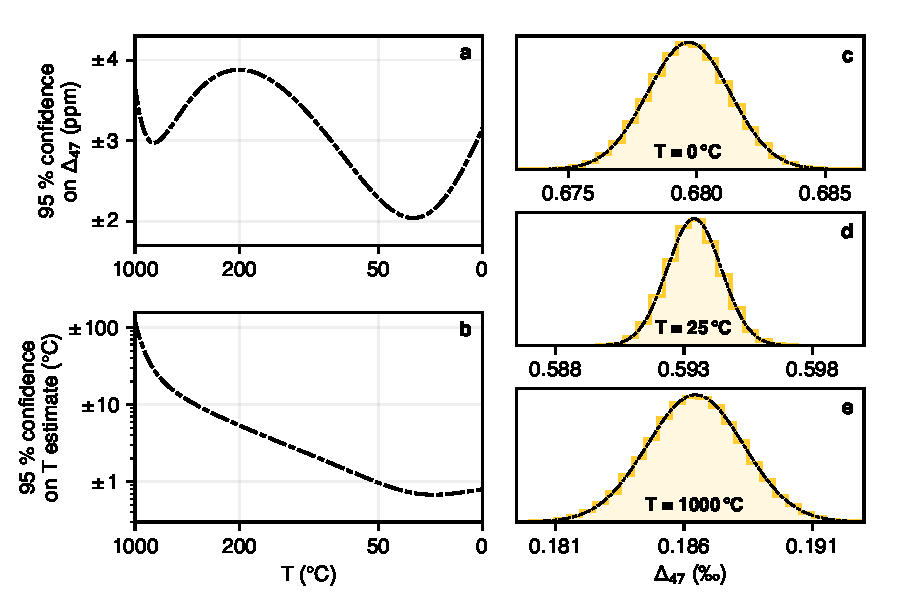
\includegraphics[width=80mm]{input/qmc}
\caption{
\textbf{Lorem ipsum dolor sit amet}: Consectetur adipiscing elit, sed do
eiusmod tempor incididunt ut labore et dolore magna aliqua. Vitae
elementum curabitur vitae nunc. Nunc lobortis mattis aliquam faucibus.
Orci sagittis eu volutpat odio. Lobortis scelerisque fermentum dui
faucibus in ornare quam viverra orci. Vitae congue eu consequat ac felis
donec. Quis risus sed vulputate odio ut enim. Pellentesque pulvinar
pellentesque habitant morbi tristique senectus et. Arcu dictum varius
duis at consectetur lorem. Fermentum dui faucibus in ornare.
}
\label{fig:qmc}
\end{figure}

\hypertarget{methods}{%
\section{Methods}\label{methods}}

\label{sec:methods}

Vitae nunc sed velit dignissim sodales. Mauris a diam maecenas sed. Sed
ullamcorper morbi tincidunt ornare massa. Ut diam quam nulla porttitor
massa id neque aliquam vestibulum. Massa sapien faucibus et molestie ac
feugiat sed. Tortor consequat id porta nibh venenatis cras. Nulla
pellentesque dignissim enim sit amet venenatis urna. Viverra nibh cras
pulvinar mattis nunc sed. Ac odio tempor orci dapibus ultrices in.
Posuere ac ut consequat semper viverra nam libero justo. Enim tortor at
auctor urna. Eu augue ut lectus arcu bibendum at varius vel pharetra.
Feugiat vivamus at augue eget arcu dictum varius duis. Mattis enim ut
tellus elementum sagittis vitae et leo. Ac ut consequat semper viverra
nam libero justo laoreet sit. Enim ut tellus elementum sagittis vitae et
leo. Amet nisl suscipit adipiscing bibendum est. Non blandit massa enim
nec dui nunc mattis enim ut. Tellus elementum sagittis vitae et leo duis
ut.

Amet commodo nulla facilisi nullam vehicula. Congue mauris rhoncus
aenean vel elit. Mattis molestie a iaculis at erat pellentesque
adipiscing commodo elit. Euismod lacinia at quis risus sed vulputate
odio. Lacinia quis vel eros donec ac odio. Mattis pellentesque id nibh
tortor id aliquet lectus. Mi proin sed libero enim sed faucibus turpis
in. Ut sem viverra aliquet eget sit amet tellus cras. Egestas diam in
arcu cursus. Enim ut sem viverra aliquet. Tortor condimentum lacinia
quis vel eros donec ac odio tempor. Tellus mauris a diam maecenas sed
enim. Mattis molestie a iaculis at erat pellentesque adipiscing commodo
elit. Lectus arcu bibendum at varius vel pharetra vel turpis nunc.

\hypertarget{results}{%
\section{Results}\label{results}}

Vivteeerra aliquet iddn section eget sit amet tellus cras. Et netus et
malesuada fames axx turpsdis \ref{sec:methods} egestas. Praesent
elementum facilisis leo vel fringilla est. Nullam ac tortor vitae purus
faucibus ornare suspendisse sed nisi. Dictum non consectetur a erat nam
at lectus urna. Facilisi etiam dignissim diam quis enim lobortis. Magna
sit amet purus gravida quis blandit. Faucibus vitae aliquet nec
ullamcorper sit amet risus nullam eget. Ultricies integer quis auctor
elit sed vulputate mi. Vestibulum lorem sed risus ultricies tristique.
Morbi tristique senectus et netus et malesuada fames. Ultricies lacus
sed turpis tincidunt id aliquet risus feugiat in. Et malesuada fames ac
turpis egestas maecenas pharetra. Nunc scelerisque viverra mauris in
aliquam sem fringilla ut morbi. At risus viverra adipiscing at in tellus
integer feugiat scelerisque. Sed ullamcorper morbi tincidunt ornare
massa eget egestas purus viverra. Eros in cursus turpis massa tincidunt
dui ut.

Bibendum ut tristique et egestas quis. Maecenas volutpat blandit aliquam
etiam erat. Velit egestas dui id ornare arcu odio. Commodo ullamcorper a
lacus vestibulum sed arcu non odio. Ut lectus arcu bibendum at varius
vel. Vitae tortor condimentum lacinia quis. Mattis nunc sed blandit
libero volutpat. Dolor sit amet consectetur adipiscing elit duis
tristique sollicitudin nibh. Est ullamcorper eget nulla facilisi. In
massa tempor nec feugiat nisl pretium fusce. At consectetur lorem donec
massa sapien. Dui sapien eget mi proin sed libero enim sed. Eget velit
aliquet sagittis id consectetur. A diam sollicitudin tempor id eu nisl.
Eleifend quam adipiscing vitae proin. Nunc mattis enim ut tellus
elementum sagittis.

\hypertarget{discussion}{%
\section{Discussion}\label{discussion}}

Feugiat vivamus at augue eget. In hendrerit gravida rutrum quisque non
tellus. Neque vitae tempus quam pellentesque. Porttitor lacus luctus
accumsan tortor posuere ac. Egestas sed tempus urna et. Suspendisse
ultrices gravida dictum fusce ut placerat orci nulla. Nisl nisi
scelerisque eu ultrices vitae auctor eu. Massa eget egestas purus
viverra accumsan in. Sit amet justo donec enim diam vulputate ut
pharetra. Ullamcorper velit sed ullamcorper morbi tincidunt. Morbi quis
commodo odio aenean. Sed adipiscing diam donec adipiscing tristique
risus nec.

Elit pellentesque habitant morbi tristique senectus et. Pellentesque nec
nam aliquam sem et tortor consequat id porta. Scelerisque viverra mauris
in aliquam sem fringilla ut morbi tincidunt. Vitae ultricies leo integer
malesuada nunc vel risus commodo. Dignissim convallis aenean et tortor
at risus viverra adipiscing. Sit amet justo donec enim. Neque aliquam
vestibulum morbi blandit cursus risus. Quis blandit turpis cursus in hac
habitasse platea dictumst. Neque aliquam vestibulum morbi blandit cursus
risus at. Et malesuada fames ac turpis egestas. Egestas erat imperdiet
sed euismod nisi porta lorem. Nisl pretium fusce id velit ut. Nisl
condimentum id venenatis a condimentum vitae sapien pellentesque
habitant. Vestibulum morbi blandit cursus risus at. Eget sit amet tellus
cras adipiscing enim. Proin nibh nisl condimentum id venenatis a
condimentum vitae sapien. Viverra nam libero justo laoreet sit amet
cursus. Metus aliquam eleifend mi in.

Neque gravida in fermentum et sollicitudin ac. Quam lacus suspendisse
faucibus interdum posuere lorem ipsum dolor. Cursus in hac habitasse
platea dictumst. Tincidunt tortor aliquam nulla facilisi cras fermentum.
Nam libero justo laoreet sit amet cursus. Sed turpis tincidunt id
aliquet risus feugiat in ante metus. Nisl condimentum id venenatis a
condimentum vitae sapien pellentesque. A cras semper auctor neque vitae
tempus quam. Mauris nunc congue nisi vitae. Donec et odio pellentesque
diam volutpat commodo sed egestas egestas. Sed ullamcorper morbi
tincidunt ornare massa eget egestas purus. Vulputate ut pharetra sit
amet aliquam id diam maecenas ultricies. Viverra orci sagittis eu
volutpat odio facilisis mauris sit. Suscipit tellus mauris a diam
maecenas sed enim ut. Venenatis cras sed felis eget velit. Tortor
pretium viverra suspendisse potenti nullam ac tortor vitae. Scelerisque
varius morbi enim nunc faucibus. Sed blandit libero volutpat sed.

\hypertarget{conclusion}{%
\section{Conclusion}\label{conclusion}}

Integer vitae justo eget magna fermentum iaculis eu non. Pulvinar mattis
nunc sed blandit libero volutpat sed. Est lorem ipsum dolor sit amet
consectetur adipiscing. Vitae suscipit tellus mauris a diam. Volutpat
blandit aliquam etiam erat velit scelerisque in dictum. Nibh mauris
cursus mattis molestie. Adipiscing elit duis tristique sollicitudin nibh
sit amet. Nunc consequat interdum varius sit amet. Eget duis at tellus
at urna condimentum mattis pellentesque id. Leo vel orci porta non
pulvinar. Adipiscing vitae proin sagittis nisl rhoncus mattis. Felis
bibendum ut tristique et egestas. Blandit cursus risus at ultrices mi
tempus imperdiet nulla malesuada. Malesuada nunc vel risus commodo
viverra maecenas. Vestibulum rhoncus est pellentesque elit ullamcorper
dignissim cras. Risus viverra adipiscing at in tellus. Duis ut diam quam
nulla porttitor. Sed cras ornare arcu dui vivamus. Sed adipiscing diam
donec adipiscing tristique risus. Turpis tincidunt id aliquet risus
feugiat in.


\IfFileExists{input/acknowledgements.tex}%
	{\subsection*{Acknowledgements}Foo bar baz.
}{}
\IfFileExists{input/contributions.tex}%
	{\subsection*{Author contributions}MD did the experiments. JC processed the data. SK drafted the
manuscript. All authors contributed to manuscript improvement and
revisions.
}{}
\IfFileExists{input/reproducibility.tex}%
	{\subsection*{Reproducible research}Foo bar baz.
}{}

\printbibliography
\end{document}